\subsection{Time Frames}
We separate the dataset into different time frames, including total time, weekday, weekend, daytime, evening time, morning\_rush hours, evening\_rush hours and travel\_hours.Fig.\ref{fig3} shows the average use-rate of the time frames above.
\begin{figure}[!htp]
	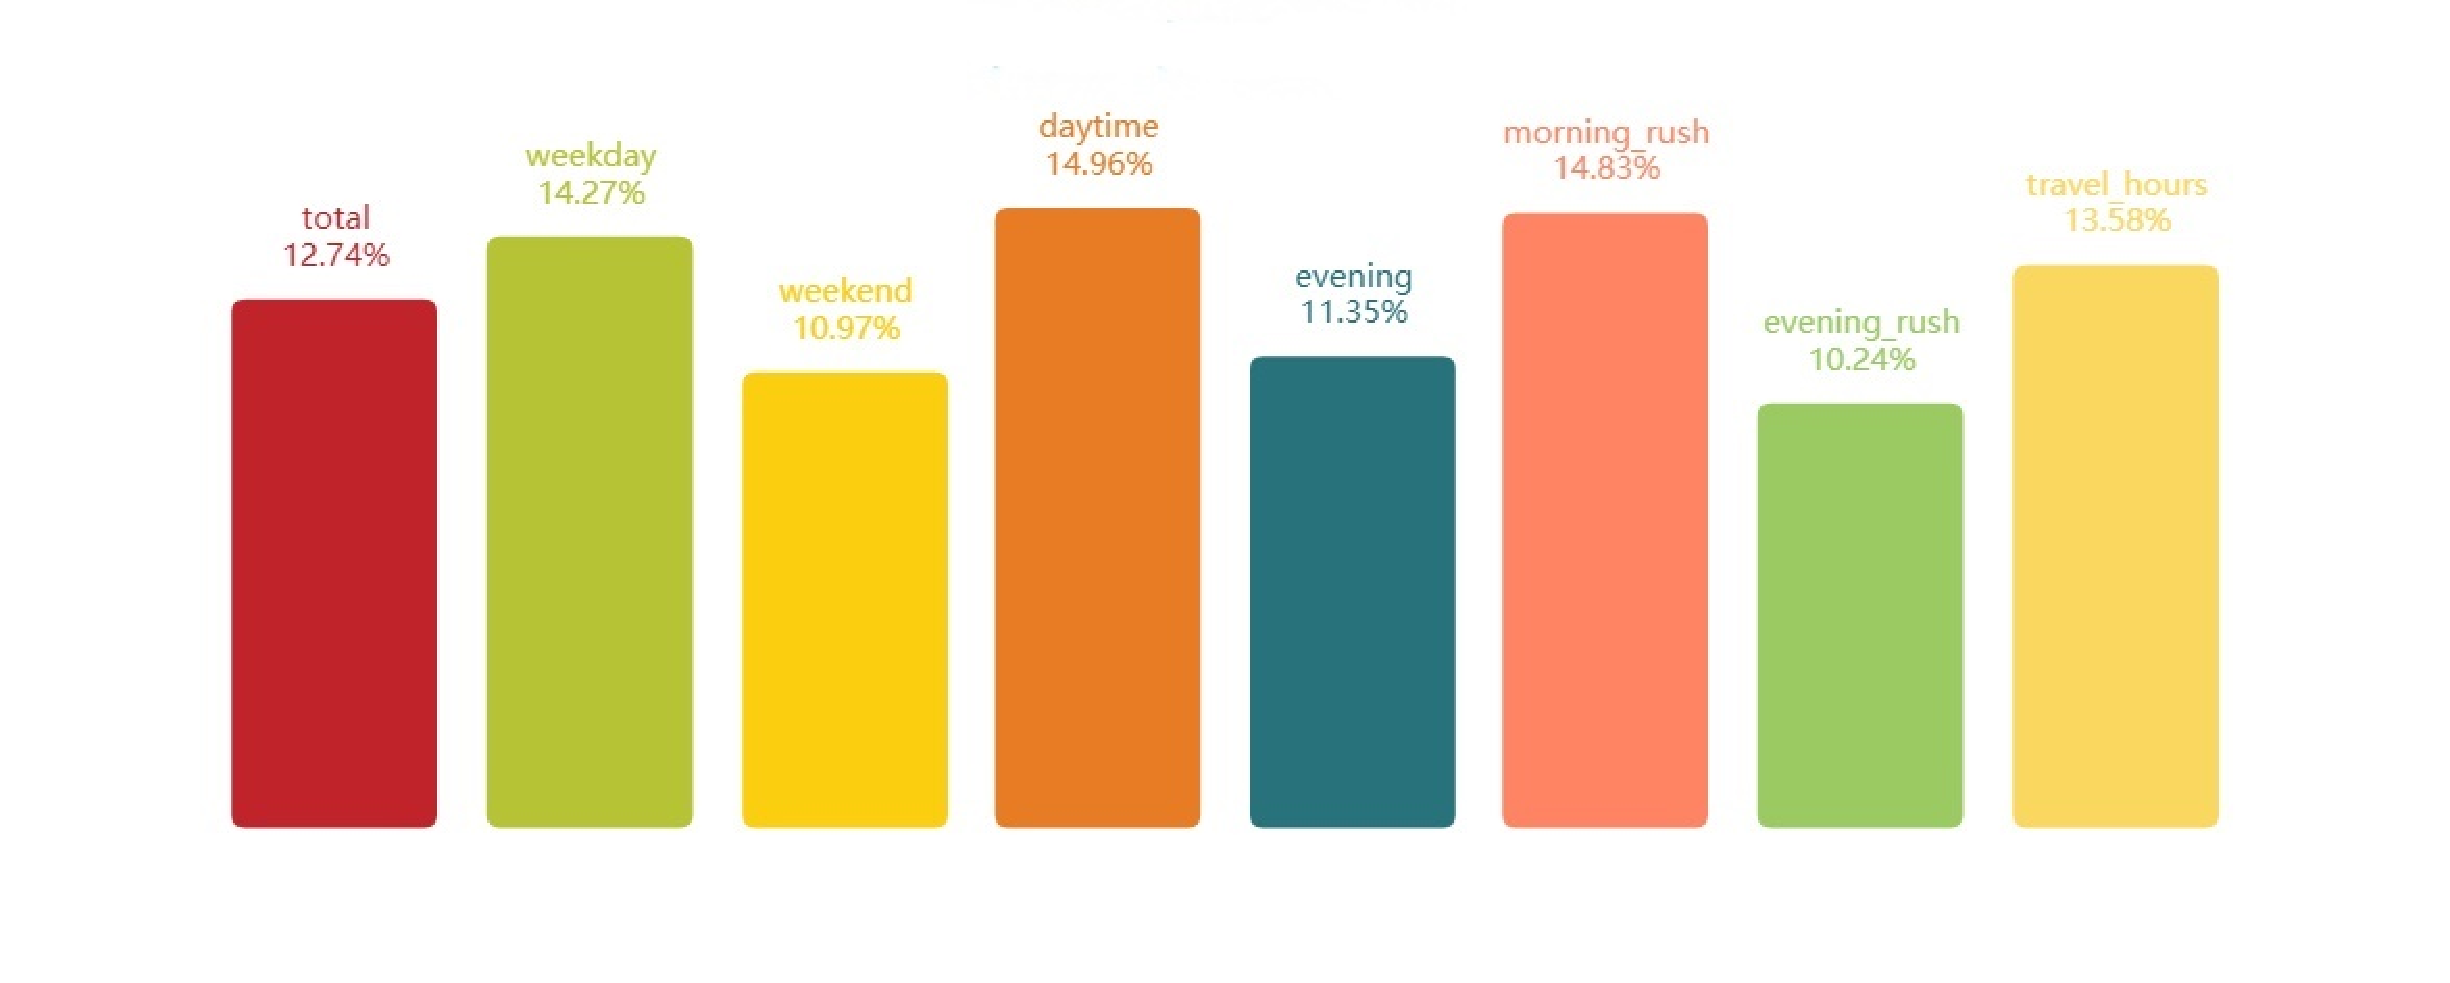
\includegraphics[width=\columnwidth]{./figures/timeframes.pdf}
	\centering
	\caption{Average use-rate of different time frames}
	\label{fig3}
\end{figure}

\subsection{Model Description}
In each time frame, we add the geographical information as well as working elements into the prediction model, in order to predict whether it’s a high use\_rate station or a low use\_rate one.
\section{Experiment}

\subsection{Datasets}
In this paper, we gather the charging stations logs from all the existing charging station companies who provide their services in Shanghai, with a total of over 2,000,000 lines. The log has a length of one month, from 2018/10 to 2018/11, in which an hourly summarize of each charging station is recorded, showing whether it's occupied or not. After preprocessing, the training set has 80\% of valid data, the test set has 20\% left.

\subsection{Implementation}

With features extracted from our collected dataset, there are mainly three groups of them, including POIs, charing price and station types, that are added into the time frame based models. Fig.\ref{fig4} shows the general flow path of our work.
=======
\subsection{Implementation}

With features extracted from our collected dataset, there are mainly three groups of them, including POIs, charing price and station types, that are added into the time frame based models. Fig.\ref{fig8} shows the general flow path of our work.
>>>>>>> update

\begin{figure}[!htp]
	\centering
		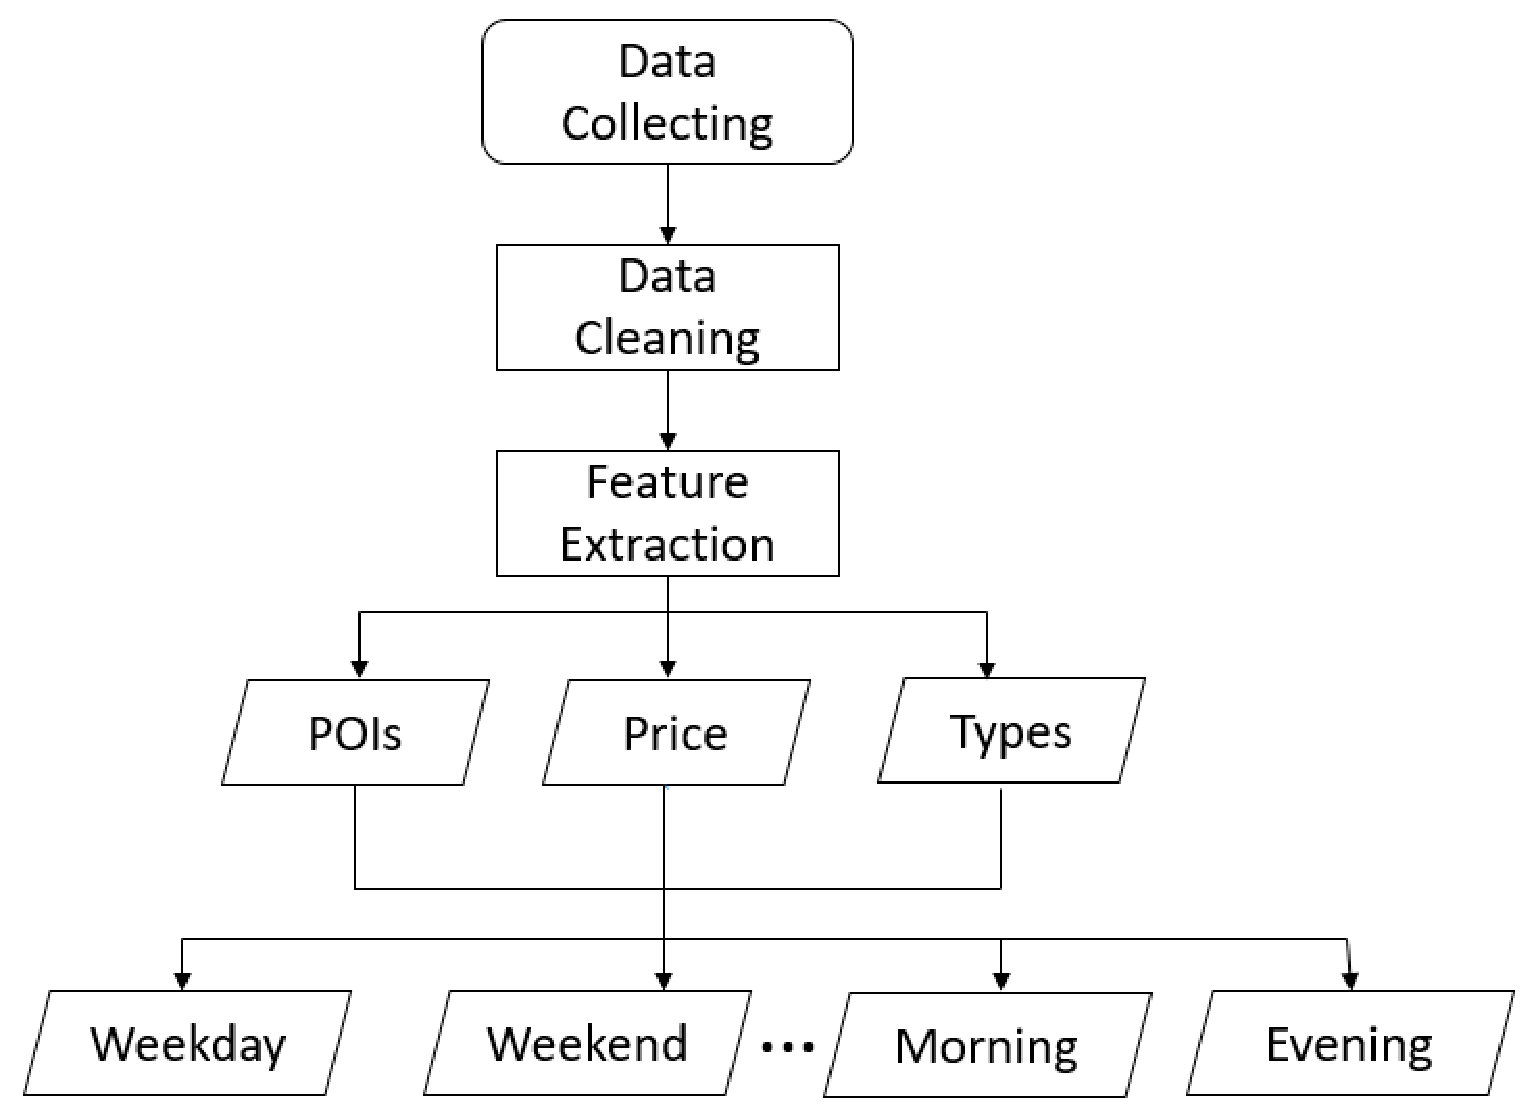
\includegraphics[width=\columnwidth]{./figures/path.pdf}
	\caption{Implementation of the work}
<<<<<<< HEAD
	\label{fig4}
=======
	\label{fig8}
>>>>>>> update
\end{figure}